\documentclass[12pt]{article}
\usepackage[english]{babel}
\usepackage[utf8x]{inputenc}
\usepackage[T1]{fontenc}
\usepackage{scribe}
\usepackage{listings}
\usepackage{mathtools}
\usepackage{listings}
\usepackage{tikz}
\usepackage{algorithm}
\usepackage{algpseudocode}
\usepackage{xcolor}

\lstdefinestyle{mystyle}{
    backgroundcolor=\color{backcolour},   
    commentstyle=\color{codegreen},
    keywordstyle=\color{magenta},
    numberstyle=\tiny\color{codegray},
    stringstyle=\color{codepurple},
    basicstyle=\ttfamily\footnotesize,
    breakatwhitespace=false,         
    breaklines=true,                 
    captionpos=b,                    
    keepspaces=true,                 
    numbers=left,                    
    numbersep=5pt,                  
    showspaces=false,                
    showstringspaces=false,
    showtabs=false,                  
    tabsize=2
}

\tikzstyle{data} = [circle, minimum size = 3 cm,text centered, draw=black, thick, fill=red!30, text=white]
\tikzstyle{model} = [rectangle, minimum width=3cm, minimum height=3cm, text centered, draw=black, fill=orange!30]
\tikzstyle{arrow} = [thick,->,>=stealth]
\tikzstyle{outp} = [rectangle, rounded corners, minimum width=3cm, minimum height=3cm,text centered, draw=black, fill=green!30]

\Scribe{Group 41 \& Group 42}
\Lecturer{Abir De}
\LectureNumber{20}
\LectureDate{27 October 2022}
\LectureTitle{Gradient Descent}

\lstset{style=mystyle}

\begin{document}
	\MakeScribeTop

%#############################################################
%#############################################################
%#############################################################
%#############################################################

% This is some warmup discussion before the first section.

% \section{Here's a section header}

% Here's some more text.
% % Here's a citation~\cite{Kar84a}.

% \subsection{Here's a subsection}

% You might like to put use subsectioning these too.  An alternate way to put in a small subheading for a paragraph is to use the \begin{verbatim} \paragraph \end{verbatim} command.  For example:

% \paragraph{A remembrance by Dantzig.}  The early days were full of intense excitement. Scientists, free at last from war-time pressures, entered the post-war period hungry for new areas of research. The computer came on the scene at just the right time. Economists and mathematicians were intrigued with the possibility that the fundamental problem of optimal allocation of scarce resources could be numerically solved. Not too long after my first meeting with Tucker there was a meeting of the Econometric Society in Wisconsin attended by well-known statisticians and mathematicians like Hotelling and von Neumann, and economists like Koopmans. I was a young unknown and I remember how frightened I was at the idea of presenting for the first time to such a distinguished audience, the concept of linear programming.



% \section{Math stuff}

% Please make an effort to typeset things nicely.  There are quite a few macros in the lpsdp.sty file.  Below are illustrated how to do some basic things; please study the \LaTeX\ carefully.

% Here's a typical LP in standard/equational form, with an equation number on one of the constraints.
% \begin{gather}
%     \min \quad c^\top x                       \nonumber\\
%     \begin{aligned}
%         \text{s.t.} \quad   Ax &= b           \nonumber\\
%                              x &\geq 0       \label{eqn:nonnegative}
%     \end{aligned}
% \end{gather}

% \noindent Here's a reference to the~\eqref{eqn:nonnegative} nonnegativity constraint.  Some more LPs:

% \begin{gather*}
%     \min \quad 3x_1 - 5x_2 \\
%     \begin{aligned}
%         \text{s.t.} \quad   x_1 + 2x_2 &\leq 6\\
%                             2x_1 + x_2 &\leq 6\\
%                             2x_1 + 2x_2 &\geq 7\\
%                             x_1,x_2 &\geq 0
%     \end{aligned}
% \end{gather*}

% \begin{alignat*}{3}
%     \text{minimize}&   \quad & 3x_1 - 5x_2 + 2x_3 - x_4&       & &\\
%     \text{subject to}& \quad & x_1 + 2x_2 - 4x_3 + x_4 &\leq 6 & &\\
%                            & & -x_1 + 3x_2 - x_3 - x_4 &\geq 7 & &\\
%                            & & x_i &\geq 0  & &\quad \forall i = 1\dots 4
% \end{alignat*}

% \begin{align}
%     & \min_{\varepsilon^{up}, \varepsilon^{dw}, \beta}  &&  \sum_{i \in Observations} {\varepsilon^{up}}_i + {\varepsilon^{dw}}_i  && \notag \\
%     & \text{subject to}     &&  {\varepsilon^{up}}_i \geq + y_i - \sum_{j \in Candidates} \beta_j x_{i,j} && \forall i \in Observations \notag \\
%     &                       &&  {\varepsilon^{dw}}_i \geq - y_i + \sum_{j \in Candidates} \beta_j x_{i,j} && \forall i \in Observations \notag \\
%     &                       &&  {\varepsilon^{up}}_i, {\varepsilon^{dw}}_i \geq 0 && \forall i \in Observations \notag \\
% \end{align}

% \begin{alignat*}{4}
% z_k(x) \ = \ & \min_{y_k}        &       &  f_k^T y_k &&                  \notag \\
%              & \text{subject to} & \quad &  D_k y_k   &&  = d_k - B_k x  \notag \\
%              &                   &       &  y_k       && \geq 0          \notag \\
% \end{alignat*}

% Huge LP's:

% \begin{align}
%     & \min_{x, y_k}     &&  c^T x && + f_1^T y_1 && + \dots && + f_n^T y_n  &&  \notag \\
%     & \text{subject to} &&  Ax    &&             &&         &&              && = b \notag \\
%     &                   &&  B_1 x && + D_1 y_1   &&         &&              && = d_1 \notag \\
%     &                   &&  \dots &&             &&  \dots  &&              &&       \notag \\
%     &                   &&  B_n x &&             &&         && + D_n y_n    && = d_n \notag \\
%     &                   &&   x,   &&     y_1,    &&         &&       y_n    && \geq 0 \notag \\
% \end{align}


% Let's do some matrices:
% \[
% \begin{pmatrix}
%     1 & \rho & \rho\\
%     \rho & 1 & \rho\\
%     \rho & \rho & 1\\
% \end{pmatrix},
% \quad \text{or alternately,} \quad
% \begin{bmatrix}
%     1 & 2 \\
%     3 & 4 \\
% \end{bmatrix}.
% \]
% More generically:
% \[
%     A = \begin{bmatrix}
%             \vrule & \vrule & & \vrule\\
%             A_{1} & A_{2} & \cdots & A_{n} \\
%             \vrule & \vrule & & \vrule
%         \end{bmatrix}
%       = \begin{bmatrix}
%             \text{---} & a_1 & \text{---} \\
%             \text{---} & a_1 & \text{---} \\
%                        & \vdots &  \\
%             \text{---} & a_n & \text{---} 
%         \end{bmatrix}
% \]


% Here's some more random typesetting: 
% \begin{itemize}
% \item ``PTIME vs. NP, where the former means time $\poly(n)$'';
% \item $\wt{O}(f(x)) \text{ is } f(x) \cdot \polylog(f(x))$;
% \item $\displaystyle 
%         g(x) = \begin{cases}
%                    \sin(2\theta) & \text{if $\theta \leq \pi$,}\\
%                    \max\{\cos^2\theta, \tfrac13\} & \text{if $\theta > \pi$.}
%                \end{cases}
%       $
% \end{itemize}
% Please don't write $max(A)$ when you mean $\max(A)$, or $log(n)$ when you mean $\log(n)$, or "quotes" when you mean ``quotes''.

% \

% More equations:

% $\max \Big\{ \sum_{i \in Observations} \Big( y_i - \sum_{j \in Candidates} \beta_j x_{i,j} \Big) ^2 \Big\}$

% $\max\Bigg\{ \sum_{i \in Observations} \Big| y_i - \sum_{j \in Candidates} \beta_j x_{i,j} \Big| \Bigg\}$

% A theorem and a proof:
% \begin{theorem} $(a+b)^2 = a^2 + 2ab + b^2$.
% \end{theorem}
% \begin{proof}
% Let for the reader.
% \end{proof}

% \bigskip

% Here's what to do if your proof ends on an equation:
% \begin{proof}
% It's easy:
% \[
%     (a+b)^2 = (a+b)(a+b) = (a+b)a + (a+b)b = a^2 + ba + ab + b^2 = a^2 + 2ab + b^2 \qedhere
% \]
% \end{proof}

% And a lemma without proof:
% \begin{lemma}
% Suppose numbers exist, then $(a+b)^2 = a^2 + 2ab + b^2$.
% \end{lemma}

% You can do a few others:
% \begin{example}
% Suppose numbers exist, then $(a+b)^2 = a^2 + 2ab + b^2$.
% \end{example}
% \begin{conjecture}
% Suppose numbers exist, then $(a+b)^2 = a^2 + 2ab + b^2$.
% \end{conjecture}
% \begin{definition}
% Suppose numbers exist, then $(a+b)^2 = a^2 + 2ab + b^2$.
% \end{definition}
% \begin{observation}
% Suppose numbers exist, then $(a+b)^2 = a^2 + 2ab + b^2$.
% \end{observation}
% \begin{remark}
% Suppose numbers exist, then $(a+b)^2 = a^2 + 2ab + b^2$.
% \end{remark}
% \begin{claim}
% Suppose numbers exist, then $(a+b)^2 = a^2 + 2ab + b^2$.
% \end{claim}



% Please insert figures liberally.  It's probably best if ``vector graphics'' are in pdf or png format, and ``bitmap graphics'' are in jpg format, but lots formats are supported.  There's a macro defined to make things easy.  Inkscape is a pretty reasonable, free program in which to draw figures.
 
% %%%%%%%% FIGURES
% % first parameter is a real number which is the scale factor; 
% % second is the file name; 
% % third is caption; 
% % fourth gives the LaTeX label for future \ref
% \myfig{.375}{example-figure.pdf}{The region $g_1 > 0, g_2 > -\tfrac{\rho}{\sqrt{1-\rho^2}}g_1$.}{fig:my-example}

% Once you've inserted it, you can refer to it as Figure~\ref{fig:my-example}.\\

% Here there is an example of some code
% \begin{lstlisting}[language=Julia]
% using JuMP, GLPK

% function production_model()
%     # Define an optimization model
%     m = Model(with_optimizer(GLPK.Optimizer))
    
%     # Variables
%     @variable(m, x[i in 1:2] >= 0)
    
%     # Constraints
%     @constraint(m, 2*x[1] + x[2] <= 4)
%     @constraint(m, x[1] + 2*x[2] <= 4)
    
%     # Objective function
%     @objective(m, Max, 4*x[1] + 3*x[3])
    
%     # Solve the model
%     optimize!(m)
    
%     return objective_value(m)
% end
% \end{lstlisting}
% Finally, if you have citations, see the commented-out stuff in the \LaTeX~here.

% \

% My farourive Optimization books are \cite{bertsimas1997introduction} \cite{boyd2004convex} \cite{wolsey2014integer}. You should add bibliographical notes in the \textbf{BibTex}: \textit{mybib.bib} file. Its good to grab these notes from Google scholar citations.

% %%%%%%%%%%% If you don't have citations then comment the lines below:
% %

Till now, we haven't discussed minimization of \textbf{Supervised Learning Algorithms yet}. In this lecture, we cover the optimisation technique \textbf{Gradient Descent}; the working of the algorithm, the cause of stochastic behaviour of gradient descent and how to utilise this stochastic nature to our advantage. We also see applications of gradient descent in an upcoming technology known as \textit{MLaaS} (\textit{M}achine \textit{L}earning \textit{a}s \textit{a} \textit{S}ervice). This lecture is mainly theoretical in nature where many concepts are just introduced at a very high level without getting into the Maths and detailed theory involved.

\section{Introduction}
Optimisation is a central requirement in machine learning. For instance, consider we have a dataset $\mathcal{D}$ with the $i^{th}$ data point $(x_i,y_i)\in \mathcal{D}$. Then, for a given model $f(x) = \theta^T x_i$ loss function, we have
\begin{gather}
    L(\theta) = \sum_{i \in \mathcal{D}} L(\theta^Tx_i,y_i)
    \intertext{And, we seek to solve the following optimisation problem}
    \min_\theta L(\theta)
\end{gather}
Let us represent the initial value of the model (the starting point) as $\theta^0$.
% We do not discuss how $\theta^0$ is chosen for the moment, but seek to find the following assurance from our optimisation algorithm
We seek the following assurance from our optimization algorithm
\begin{gather*}
    \theta^0 \xrightarrow[]{???} \theta^\ast = \arg\min_\theta L(\theta)
\end{gather*}
Thus, whatever the initial value of the weights/learnable parameter ($\theta^0$), we obtain $\theta^\ast$

We now answer some crucial questions about $\theta^0$ such as:
\begin{itemize}
    \item How do we choose $\theta^0$ and what effect does this choice have on our results?
    \item Do we converge to `the' minima on starting from any $\theta^0$?
\end{itemize}

\section{The Gradient Descent Setup}
Gradient Descent begins with a starting value, $\theta^0$. Then, at each intermediate value of the model, it computes the gradient of the loss function with respect to the model parameters and updates the model a fixed constant (called learning rate) times the gradient in the 'direction' opposite to that of the gradient. Thus, we express
\begin{gather}
    \theta^t = \theta^{t-1} - \eta_t \nabla_\theta L(\theta)
\end{gather}
where $\eta_n$ is the learning rate at time step `$t$' and $\theta^t$ represents the model weights/parameters after `$t$' iterations and we terminate when a suitable convergence condition is met. The value of $\theta$ thus obtained is claimed to be $\theta^\ast$ 

The aim of gradient descent (GD) algorithms is to minimize function $l$ with respect to parameters $\mathbf{w}$ by updating them towards negative gradient. Whether the algorithm converges to a global or local minimum, or at all, depends on the initialization of parameters, step size (= learning rate), and properties of the loss function such as convexity. 
\\
The pseudocode for GD is as follows :
\begin{algorithm}
  \caption{Gradient Descent}\label{gd}
  \begin{algorithmic}[1]
      \State $\mathbf{w}_0 \gets \mathbf{r}$\Comment{$\mathbf{r}$ is a randomly initialised vector}
      \State $i \gets 0$
      \While{(\texttt{$\mathbf{w}$ has not converged})}
        \State $\mathbf{w}_{i+1} \gets \mathbf{w}_i - \eta_i \cdot \text{Grad}(\ell, \mathbf{w}_i, \mathbf{x}, \mathbf{y})$
        \State $i \gets i+1$
      \EndWhile\label{gdwhile}
  \end{algorithmic}
\end{algorithm}\\
Here, Grad($\cdot$) is substituted according to the algorithms being GD, Mini-batch GD or SGD.
Note that the hyperparameters $\mathbf{w}_0$ and $\eta$ can be tuned and affect the speed as well as convergence result of the algorithm (in finite steps).


\subsection{Vanilla/Batch Gradient descent}
When the number of training samples is relatively small, an effective method to update the parameters is to compute the gradient using the whole training set at each iteration:
\begin{align*}
    \mathbf{w}_{i+1} &= \mathbf{w}_i - \eta_i \nabla_w l(\mathbf{w}_i)\\
    &= \mathbf{w}_i - \eta_i \sum_{(x, y)\in \mathcal{D}} \nabla_w \ell(\mathbf{w}_i,\mathbf{x},\mathbf{y})
\end{align*}
where $\eta_i$ is the learning rate. Note that the learning rate does not necessarily have to be constant during the search. Even though batch GD converges with comparably small number of iterations,
calculating the gradient with a large training set can be  computationally very inefficient.

\textbf{Note}: This is also referred to as Batch Gradient Descent in multiple texts.

\subsection{Mini-batch gradient descent}
In mini-batch GD, the gradient is computed by using a smaller subsets of the training set at each iteration. If $B_1, B_2, ... \subset \mathcal{D}$, is a partition of the training set, then the parameters are updated by
\begin{equation*}
\mathbf{w}_{i+1} = \mathbf{w}_i - \eta_i \sum_{(x,y) \in \B_i} \nabla_w\ell(\mathbf{w}_i,\mathbf{x},\mathbf{y})
\end{equation*}
It is likely that the algorithm does not converge before using all the batches, and in this case the batches are shuffled and re-iterated.
\\
When the size of dataset is large it is a difficult job to store the gradients calculated using all of the training instances. This is a limitation caused due to the \textbf{GPU memory}.

To resolve this issue, mini-batch GD is adopted with a feasible batch size (practically, it is around 10-20 for Computer Vision applications with 360p image resolutions and 2-4 in NLP applications involving documents). It improves the speed of convergence as well since quicker (but noisier) updates are made to the parameters.

\subsection{Stochastic gradient descent}
In stochastic GD, the training set is shuffled and the gradient is computed using a single (random) instance at each step. In every iteration, the training set is randomly shuffled and such updates are performed for all instances :
\begin{align*}
\mathbf{w} = \mathbf{w} - \eta_i \nabla_w\ell(\mathbf{w},\mathbf{x},\mathbf{y})
\end{align*}
where $(\mathbf{x}, \mathbf{y})$ is the random instance for one of the updates. In this algorithm, it is not needed that the updates are along the direction of gradient vector but the expectation of updates (for every pass over the training set) is parallel to the gradient.

% \myfig{.6}{gradDes.png}{Various gradient descent algorithms}{fig:grad-desc}

\begin{figure}[H]
    \centering
    \includegraphics[width=0.65\textwidth]{gradDes.png}
\end{figure}


The figure above compares the three algorithms in their descent trends. To recall, Batch GD considers all of the training set, Mini-Batch GD considers small batches of training instances, Stochastic GD considers only single instances for gradient updates. Thus, the direction along which the update vector ($\Delta{\mathbf{w}}$ term) points and the smoothness of the descent can be explained.


\subsection{Hyper-parameters}
There are 2 hyperparameters which gradient descent needs, namely the starting point $\theta^0$ and the learning rate $\eta_t$ (possibly variable as a function of t)

\subsubsection{Choice of Learning Rate $\eta$}
This famous graph below\cite{class} that shows how a learning rate that is too big or too small affects the loss during training.

\myfig{.375}{lr.jpeg}{Choice of Learning Rate $\eta$}{fig:my-example}

With low learning rates the improvements will be linear. With high learning rates they will start to look more exponential. Higher learning rates will decay the loss faster, but they get stuck at worse values of loss (green line).

\subsubsection{Choice of $\theta^0$}
We observe, and can show, that for a given learning rate, the various values of $\theta^0$ can give different values of $\theta^\ast$. An important question lies ahead. Suppose we choose various values of the starting model, say \[\Theta^0 = \{\theta^0_1,\theta^0_2 \cdots \theta^0_n\}\] and run gradient descent to obtain the corresponding optimal values (for which loss is minimised) as \[\Theta^\ast = \{\theta^\ast_1,\theta^\ast_2 \cdots \theta^\ast_n\}\]

\myfig{.675}{loss.png}{Plot of Loss(z-axis) vs $\theta_1$(x-axis), $\theta_2$(y-axis)}{fig:loss-example}

Should we choose the best value in $\Theta^\ast$ or the average value and why?

\begin{claim}
In case of various optimal values $\theta^\ast$ corresponding to various starting values, $\theta^0$, we choose the best value of $\theta^\ast$ (for which loss is minimised)
\end{claim}

A justification to this is that, the choice of initial value can result in the gradient descent algorithm converging to a local minima and not being able to identify a ``better'' minima. Thus, the choice of various starting points allows the algorithm to explore various minima points and then choosing the best allows us to choose the more optimal value. \\
Note: The comparisons are done on the basis of performance on the \textbf{validation set}.

\subsection{Initialisation During Coding}
    \begin{itemize}
        \item Let us assume that we run optimisation multiple times, starting with random $\mathbf{w}_0^1, \mathbf{w}_0^2, \ldots$ each time resulting in validation errors as $\epsilon_1, \epsilon_2, \ldots$
        \\
        \textbf{Question}: How do we +decide which $\mathbf{w}_0^i$ to rely upon?\\
        \textbf{Claim}: Choose that $\mathbf{w}_0^i$ which gives least validation error $\epsilon_i$.\\
        \textbf{Justification}: As explained above, lower validation error means better generalisation and weights giving least error signify the (yet) best found minima.
        
        \item In mini-batch gradient descent fix the initial weight parameter $\mathbf{w}_0$ and train over various batch sequences $\{\mathcal{B}_0^i, \mathcal{B}_1^i, \mathcal{B}_2^i, \ldots\}_{i = 0}^N$\\
        Assume that $\mathbf{w}_0$ generates error $\epsilon_i$ for the $i$th sequence 
        \\
        \textbf{Question}: While comparing various initialisations of $\mathbf{w}_0$, what metric should we use to judge them? Best error i.e. $\min(\mathbf{\epsilon}_i)$ or average error i.e. $\bar{\epsilon}$?\\
        \textbf{Claim}: Use the average error i.e. $\bar{\epsilon}$ and not $\min(\epsilon_i)$ as a judging metric\\
        \textbf{Justification}: Relying on the sequence of batches is equivalent to using validation for training the model and this results in overfitting. Average error is equivalent to $\mathbb{E}[\mathbf{\epsilon}]$ when a large \#batches are tried and is a better way to judge the parameter.
        
        \item \textbf{Question}: Where exactly do ML libraries initialise the weights?\\
They would be initialised for an instance of the model when the model object constructor is called. The parameters can also be sampled from various distributions.\cite{he}

\begin{lstlisting}[language=Python]
class MyModel(self, ...):
    
    def __init__:
        self.linear = nn.Linear(in_features, out_features)  
        #This is the line where initialization occurs with RANDOM weights
        
    def initialize(self):
        self.linear.weight.data = torch.randn(size)
        self.linear.bias.data = torch.randn(size)
        #This is the function where we initialize weights and biases according to the distribution of our choice
        
if __name__ == "__main__":
    model_instance = MyModel(...)
    #Writing this is fine, it still allows random initialization of weights
    model_instance.initialize()
    #This is optional, we write it only if we want to initialize weights with a distribution of our choice
\end{lstlisting}

We have mentioned that \texttt{Torch} automatically initializes weights of the Linear Layer when we create an instance of \texttt{nn.Linear}. One might ask what distribution did \texttt{Torch} use when it initialized the weights. \\
\texttt{Torch} uses $\mathcal{U}(-\sqrt{k}, \sqrt{k})$, where $k = \frac{1}{\text{in\_features}}$ to sample the weights. \\
Practically, we often observe a certain randomness in our results even when we use the same hyperparameters and model. What are the sources of this randomness?
\begin{enumerate}
    \item When we use \textbf{Batch Gradient Descent}, we use the gradients of the \textit{entire dataset} to move one step. That is, we will compute the gradient of loss with contribution from each point of the dataset and move in the direction opposite to this computed gradient. In such a scenario, the only source of randomness in a model (assuming we are not using other stochastic techniques such as \textbf{dropout}) is the \textit{initialization of $\theta^0$}
    \item When we use \textbf{Mini-Batch Gradient Descent}, the choice of batches is also a source of randomness which has an effect on the final outcome. In each iteration, we choose different partitions of the data set to make batches and these partitions are often random, which results in non-determinism. 
\end{enumerate}
    \end{itemize}

\section{Mini-Batch Gradient Descent}
Above, we would compute the loss function over the entire dataset, however, this suffers from one major problem; it is \textbf{slow to converge}\cite{rate}. Hence, it is prudent to use batching; training on chunks of the dataset at a time.

\subsection{Dependence on Batch Order}
We observe that the various orders of batches can give different values of $\theta^\ast$. An important question lies ahead. Suppose we choose various batch orders of the starting model, say \[\Omega = \{O_1, O_2 \cdots O_n\}\] and run gradient descent to obtain the corresponding optimal values (for which loss is minimised) as \[\Theta^\ast = \{\theta^\ast_1,\theta^\ast_2 \cdots \theta^\ast_n\}\]

Should we choose the best value in $\Theta^\ast$? Or the average value and why?

\begin{claim}
In case of various optimal values $\theta^\ast$ corresponding to various batch orders, $\theta^0$, we choose the average value of $\theta^\ast$ (for which loss is minimised)
\end{claim}

A justification to this is that, the choice of `best' batch order depends on the validation dataset and can result in the gradient descent algorithm overfitting on the validation dataset. Even if we employ early stopping to prevent overfitting on the training set, we will overfit on the validation set, since we're trying to `train' the batch choice on the validation set. For it to generalise well, we choose the average over all the optimal values obtained through the various batch orders.

We should have a \textbf{high generalization} on the validation set. If on changing batches, we get a huge change in validation error, that means the model is \textbf{not stable with respect to batches} and in that case, one should change the model or tune some other hyperparameters. 

\subsubsection{Questions to Think about on this topic}
\begin{enumerate}
    \item Can you prove an equivalence between L-2 Regularization and mini-batch gradient descent? Mini-batch gradient descent can also be used to prevent overfitting like L-2 regularization. We can say that under certain conditions, mini-batch gradient descent gives us similar results on running optimization algorithms. Can you find this strong connection?
    \item Suppose you have a 24 Gigabyte GPU and you wish to run a training algorithm with 500 epochs at max. Assume that other parameters are given, then how would you choose your batch choice?
\end{enumerate}


\section{Machine Learning as a Service}
Have you ever used a service which has an online chatbot? Say, on a banking website which employ models which use NLP techniques in creating such chatbots. MLaaS is a cloud computing service in which clients can use powerful models for their own use without having the hassle of research and development.

We will work with the simplified example of an online service which performs a certain task, say Google Translate, a service which takes an English sentence and converts it to Hindi. \\
The task is performed by a model \textit{M} trained on a large dataset $\mathcal{D}$. 
\vspace{1cm}

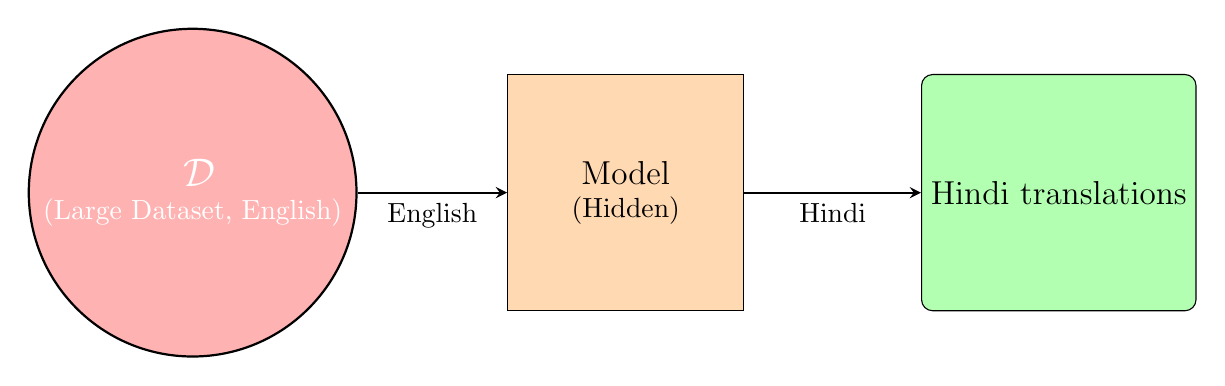
\begin{tikzpicture}
\node[data, align=center] (D) at (0,0){\begin{Large} $\mathcal{D}$\end{Large} \\ (Large Dataset, English)};
\node[model, right of=D, xshift=4.5cm, align=center] (M){\large Model \\ (Hidden)};
\node (O) [outp, right of=M, xshift=4.5cm, align=center] {\large Hindi translations};
\draw [arrow] (D) -- node[anchor=north] {English} (M); 
\draw [arrow] (M) -- node[anchor=north] {Hindi} (O);

\end{tikzpicture}
\vspace{1cm}

Now, we want to train another model \textit{M'} on a smaller dataset $\mathcal{D}'$ supplementing training using model \textit{M}, which acts as a black box since we do not have access to the internal structure and parameters of the model itself. The structure of \textit{M} is the company's trade secret. We also do not have a dataset as large as Google does!

\vspace{1cm}

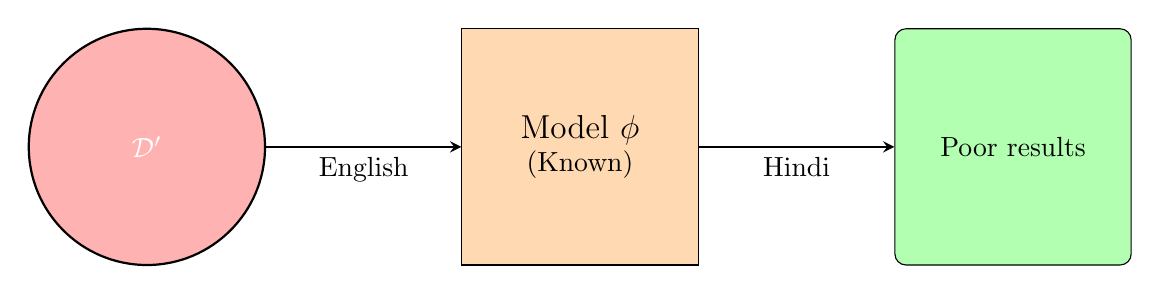
\begin{tikzpicture}
\node[data, align=center] (D') at (0,0){$\mathcal{D'}$};
\node[model, right of=D', xshift=4.5cm, align=center] (M'){\large Model $\phi$\\ (Known)};
\node (O') [outp, right of=M', xshift=4.5cm, align=center] {Poor results};
\draw [arrow] (D') -- node[anchor=north] {English} (M'); 
\draw [arrow] (M') -- node[anchor=north] {Hindi} (O');

\end{tikzpicture}
\vspace{1cm}

We wish to utilise the output of the model M during the training of M' to improve the results we would have got only using M'. \\
\textbf{Our goal is to get a `Gold Standard' output, which we call \textit{Hindi*}. Note that this is different from the translations which just Google's model gives, which is why we were employing our model in the first place. Ideal output matching \textit{Hindi*} cannot be obtained with just our data and model alone as well though. }\\

\vspace{1cm}

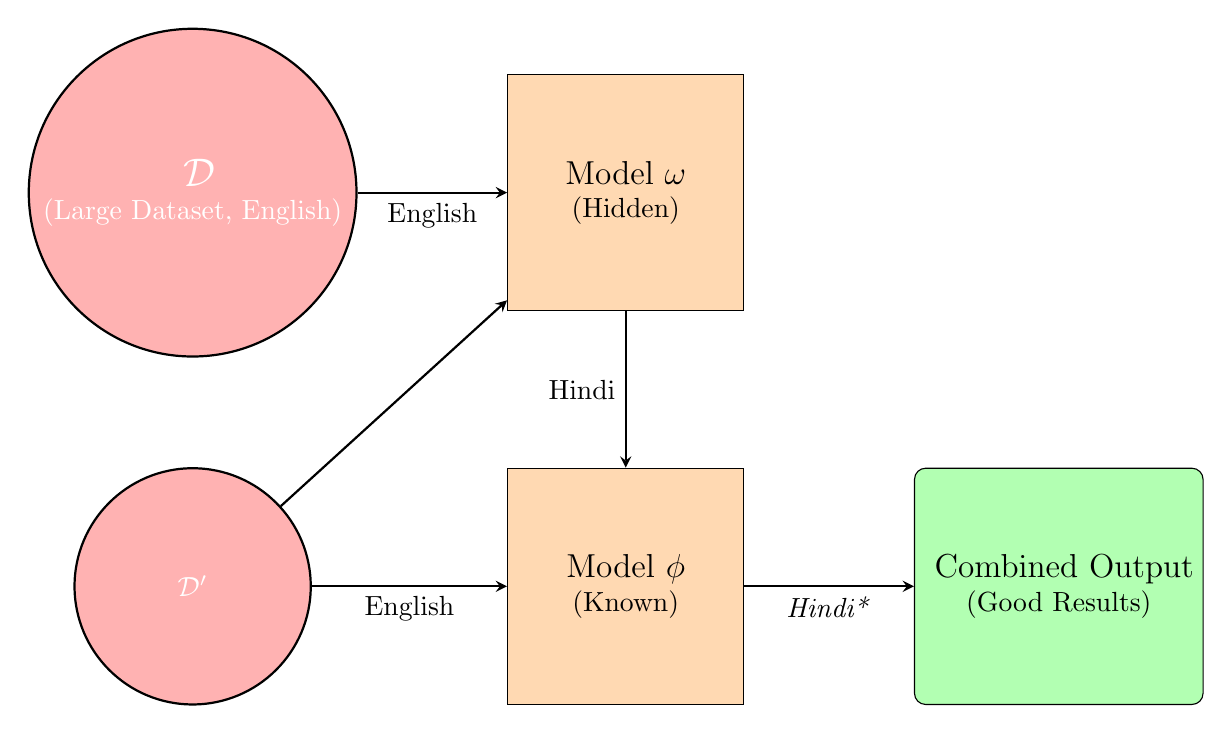
\begin{tikzpicture}
\node[data, align=center] (D) at (0,0){\begin{Large} $\mathcal{D}$\end{Large} \\ (Large Dataset, English)};
\node[model, right of=D, xshift=4.5cm, align=center] (M){\large Model $\omega$ \\ (Hidden)};
\node[data, below of=D, yshift=-4cm, align=center] (D'){$\mathcal{D'}$};
\node[model, right of=D', xshift=4.5cm, align=center] (M'){\large Model $\phi$\\ (Known)};
\draw [arrow] (D) -- node[anchor=north] {English} (M);
\draw [arrow] (D') -- node[anchor=north] {English} (M');
\draw [arrow] (M) -- node[anchor=east] {Hindi} (M');
\draw [arrow] (D') -- node[anchor=north east] {} (M);
\node (O') [outp, right of=M', xshift=4.5cm, align=center] {\begin{large} Combined Output \end{large}\\(Good Results)};
\draw [arrow] (M') -- node[anchor=north] {\textit{Hindi*}} (O');

\end{tikzpicture}

\begin{center}
    {\LARGE $\theta = \left[ \phi, \omega \right]$}\\
    {\LARGE but Learnable parameters are just $\displaystyle \phi $}
\end{center}
\vspace{1cm}

The issue is that, we cannot backpropagate through \textit{M} since the gradient of the loss with respect to the parameters of \textit{M} is not known, i.e. even though $\phi$ are known, $\phi$ and thus $\theta$ aren't. Are main problem is the lack of knowledge about the functional form of $\omega$ due to which we cannot compute gradients with respect to them. So what is the solution?

\subsubsection{Approach 1: Perturbation}
A proposed solution was that we can perturb the inputs to \textit{M} a little, thus effectively estimating the loss function around the inputs allowing us to backpropagate without knowing the gradient. This is like numerical estimation of the derivative. However, this is \textbf{very costly} since we need a huge number of queries to get smooth derivatives, numerical derivative computation is computationally expensive and thus \textbf{not a feasible solution}.

\subsubsection{Approach 2: Gaussian Processes}
The idea is to model \textit{M} using a Gaussian process (any Bayesian model can suffice), i.e. replace the entire black box by a Gaussian Process. We use this to obtain correct results and reduce uncertainty. The procedure is roughly as follows
\begin{itemize}
    \item Select an example sentence \textit{s} through $\mathcal{D}$, pass it through \textit{M} and get loss
    \item Make Gaussian process and train \textit{M'} to fine tune for sentences \textit{s'} close to original example sentence s
\end{itemize}
Using Gaussian Processes saves us the entire hassle of computing derivatives, since no derivatives are involved in Gaussian Process, thus solving our problem with backpropagation. 

Note that for a large amount of data, the \textbf{interpolative nature} of Gaussian Process almost approximates the black box we are trying to model.

\subsection{Prompt Engineering}
This is a very interesting and upcoming area of NLP. Usually a model is designed for one task. But, we can make models which can generalise to many tasks. Say, a model is trained on some set of tasks (using 1 million training samples) but tested on other task, not in the set of tasks in the training set. It is possible to provide some examples (10\footnote{Not exact numbers. Just an order of magnitude}) and retrain to make it ‘adjust’ to the new task.

As an example, suppose we are designing a complex model which processes a set of questions which are of a similar type:
\begin{enumerate}
    \item Who is the Chancellor of Germany? \textit{Ans: Olaf Scholz}
    \item When did Armstrong land on the moon? \textit{Ans: 1969}
    \item When was Obama born? \textit{Ans: 1961}
\end{enumerate}
We have a `training' data set of 1 million questions and label answers. While testing, now we give our model some 10 test examples which are nothing like what we've seen before. \\
As an example, we prompt the model, ``What is the sentiment of the people towards an X political party?" 
Although our model will not be able to answer it accurately from the training it has received, when we retrain it with \textbf{just these 10 new `test examples' (since they are not from an actual test set in the conventional set)}, the model is seen to perform surprisingly well on unseen examples. 

Have you ever heard about the godly transformer model \textbf{GPT-3}?
\\
It is a NL model that can do absolutely any task given to it in writing.
There's a huge variety of tasks that it can perform. Keeping digression aside, here the input that we provided to the model "\textit{Find the derivative of log(x)}" is called the \textbf{prompt} and then processes it.
\\
In prompt engineering, the description of the task is embedded in the input, e.g., as a question instead of it being implicitly given. Prompt engineering typically works by converting one or more tasks to a prompt-based dataset and training a language model with what has been called "prompt-based learning" or just "prompt learning". Prompt engineering may work from a large "frozen" pretrained language model and where only the representation of the prompt is learned, with what has been called "prefix-tuning" or "prompt tuning".
\\
Another way is, instead of a single sentence as a prompt, give few examples of \textbf{question-answer pairs} followed by the main question as your prompt. Then, the model interpretes the examples and owing to its huge recalling capability, is able to correctly answer your question. This is called \textbf{Few Shot Learning}.


Thus, there exists a certain robustness in the model by which when we train on a very small `test set', we will be able to \textbf{update our weights} and still get very good answers for unseen questions. This is an interesting topic of current research known as \textbf{Prompt Engineering}. 



\section{Questions to ponder}
\begin{itemize}
    \item Why the configuration/permutation of the sequence of mini-batches is not a hyperparameter but the number of bathces (in the sequence) is?
    \item Show that Gradient Descent with L2 regularization is equivalent to Mini-batch Gradient Descent without L2 regularization with some appropriate batch size.
    \item If you have a GPU with 24GB RAM and you will train a model for 500 iterations at max, then what should be the batch size you would use?
\end{itemize}

\section{Conclusion}
Gradient descent is a first-order iterative optimization algorithm for finding the minimum of a function. It is a helpful tool in the machine learning toolkit which also works moderately well in practice. There exist many gradient descent algorithms\cite{graddesc} which further optimise gradient descent. We use gradient descent to optimise models in machine learning services and prompt engineering as well


 \bibliographystyle{abbrv}           % if you need a bibliography
 \bibliography{mybib}                % assuming yours is named mybib.bib


\end{document}